\documentclass[11pt]{article}

\usepackage[margin=0.9in]{geometry}
\usepackage[T1]{fontenc}
\usepackage[utf8]{inputenc}
\usepackage{lmodern}
\usepackage{graphicx}
\usepackage{amsmath,amssymb,amsfonts}
\usepackage{textcomp}
\usepackage{xcolor}
\usepackage[hidelinks]{hyperref}
\usepackage{booktabs}
\usepackage{enumitem}
\usepackage{tikz}
\usetikzlibrary{positioning, arrows.meta, fit, calc}

\hyphenation{nano-chat permu-tational dual-stream pre-residual un-embed-der}

\setlength{\parskip}{1pt}
\setlength{\textfloatsep}{4pt plus 2pt minus 2pt}
\setlength{\intextsep}{4pt plus 2pt minus 2pt}
\usepackage{titlesec}
\titlespacing*{\section}{0pt}{8pt plus 2pt minus 2pt}{4pt}
\titlespacing*{\paragraph}{0pt}{4pt plus 1pt minus 1pt}{6pt}

\begin{document}

\title{\Large\textbf{A tiny dual-stream LUT transformer that closes most of the gap to vanilla}\\[2pt]
\large A report on the \texttt{exp304--exp430} arc, centred on \texttt{exp428}}
\author{Anatoly Starostin}
\date{}
\maketitle
\vspace{-12pt}

\noindent\textbf{Scope.}
This report continues the May 2026 status report and the short \texttt{exp303} report.
It covers the roughly one hundred and thirty experiments that followed \texttt{exp303} (\texttt{exp304} -- \texttt{exp430}), organised around the architectural and methodological shifts that produced \texttt{exp428} -- our current best LUT model on the matched 8K-step, $b{=}16$ budget.
We assume the reader is familiar with the \texttt{TinyMultiHeadLut} primitive, the single-stream and dual-stream variants from the prior reports, and the \texttt{nanochat} BPE setup ($V{=}32{,}768$, ClimbMix data, $T{=}512$, validation reported as bits per byte).

% ======================================================================
\section{Where we left off, and what changed}
\label{sec:context}

The \texttt{exp303} report introduced the dual-stream LUT transformer: an $E{=}64$ ranking carrier between blocks, alongside a $D{=}384$ real-valued residual stream fed by a per-block \texttt{residual\_lut}, with a single linear unembedder $\mathbb{R}^D \to \mathbb{R}^V$ replacing the wide concat-MLP unembedder of the single-stream model.
At 8K steps, $b{=}8$, that model finished at $1.6509$ bpb -- within $0.04$ bpb of the single-stream LUT but still behind even the vanilla MinimalGPT baseline (\texttt{exp001}: $1.6256$).

Five things changed between \texttt{exp303} and \texttt{exp428}, each addressed in its own section below:

\begin{enumerate}[itemsep=1pt, topsep=2pt]
\item The vanilla baseline was rebuilt with rotary positions; the bar is now $1.388$ bpb at 8K / $b{=}16$, not $1.626$.
\item We stopped trying to scale parameter count and committed to models of $\le 100$\,M parameters.
\item We characterised the NAP--batch trade-off: small NAP gives denser gradients, large NAP gives more expressivity, and the sweet spot is NAP $\in [4, 6]$.
\item The dual-stream block was redesigned with an identity skip on the $E$-stream (pre-norm GPT-2 style) and a fused $\mathtt{qkv\_lut}$ producing $Q$, $K$, and a shallow $V$-branch; \texttt{exp428} is the head of that lineage and crosses $1.5$ bpb at $b{=}16$, 8K.
\item Two side-quests -- distillation from a trained vanilla model, and engineering a better LUT backward pass -- did not yield improvements.
\end{enumerate}
The rest of the report walks each of these in order, then ends with the standalone bandwidth comparison and our reading of the result.

% ======================================================================
\section{Vanilla, refreshed: RoPE moves the baseline}
\label{sec:rope}

Up to \texttt{exp303}, all bpb claims were anchored to \texttt{exp001} -- vanilla MinimalGPT with learned absolute positional embeddings.
Replacing absolute positions with RoPE \emph{inside} attention, with no other change, drops val bpb from $1.626$ to $1.547$ at $b{=}8$ (\texttt{exp319}) and to $\mathbf{1.388}$ at $b{=}16$ (\texttt{exp328}); 24K steps at $b{=}16$ takes the same configuration to $1.253$ (\texttt{exp416}).

\begin{center}\small
\begin{tabular}{llrrrr}
\toprule
Run & Config & Pos.\ emb.\ & batch & steps & val bpb \\
\midrule
\texttt{exp001} & MinimalGPT 23\,M & learned abs.\ & 8  & 8K  & $1.6256$ \\
\texttt{exp319} & + RoPE           & rotary        & 8  & 8K  & $1.5468$ \\
\texttt{exp328} & + RoPE           & rotary        & 16 & 8K  & $\mathbf{1.3882}$ \\
\texttt{exp416} & + RoPE           & rotary        & 16 & 24K & $\mathbf{1.2527}$ \\
\bottomrule
\end{tabular}
\end{center}

The same modification, dropped into the LUT trunk, also helps without any further tuning -- every LUT result quoted later in this report uses RoPE on $(q, k)$ after the per-head $\mathtt{q\_norm}, \mathtt{k\_norm}$ LayerNorms.
The simplicity-vs-payoff ratio is high enough that we follow Occam's razor and treat RoPE-vanilla at $b{=}16$, 8K as the new baseline; all subsequent LUT comparisons in this report use it.

% ======================================================================
\section{Why $\le 100$\,M: the tiny-model thesis}
\label{sec:tiny}

\paragraph{Hypothesis.}
The single-stream LUT models from the May report were large (358M for \texttt{exp265}); the dual-stream \texttt{exp303} grew to 602M without overtaking vanilla.
We asked the inverse question: how small can a LUT-LM be and still be competitive with vanilla on the same batch and step budget?
Two practical reasons motivated this:
\textbf{(i)} the bandwidth story of the LUT primitive is most clearly told at modest parameter counts (Section~\ref{sec:bandwidth}), and
\textbf{(ii)} large LUTs train slowly -- as long as our bpb is dominated by the unembedder, growing the trunk is not where the gain lives.

\paragraph{TinyLUT-LM sweep.}
\texttt{exp329} -- \texttt{exp342} reset the architecture to a $22$\,M starting point and swept $E$ and $H$ at fixed batch and recipe.
The picture (Table~\ref{tab:tiny}) is consistent: parameter matching alone does not buy bpb.
A $22$\,M LUT-LM lands at $1.755$ bpb while the same-budget vanilla is at $1.388$; widening to $50$\,M closes about a third of that gap.
Beyond $\sim 100$\,M parameters, table-count increments give diminishing per-parameter returns -- so we capped the design space there and put all further effort into recipe and architecture.

\begin{table}[!ht]
\caption{Tiny-LUT parameter sweep (8K steps, $b{=}16$, LUT trunk only). \texttt{exp329} is the seed configuration; the rest vary a single knob. Vanilla \texttt{exp328} at 23\,M is included as the reference at matched budget.}
\label{tab:tiny}
\centering\small
\begin{tabular}{llrrl}
\toprule
Run & Knob & Params & val bpb & $\Delta$ vs.\ vanilla 23\,M \\
\midrule
\texttt{exp328} & vanilla + RoPE          & $23.4$\,M & $1.388$ & --- \\
\midrule
\texttt{exp329} & TinyLUT seed            & $21.8$\,M & $1.755$ & $+0.367$ \\
\texttt{exp339} & $E{=}48$                & $38.3$\,M & $1.654$ & $+0.266$ \\
\texttt{exp340} & $E{=}48$ + out\_tph$\,128$    & $43.1$\,M & $1.637$ & $+0.249$ \\
\texttt{exp338} & $E{=}96$                & $44.6$\,M & $1.646$ & $+0.258$ \\
\texttt{exp342} & $H{=}12$                & $50.5$\,M & $1.634$ & $+0.246$ \\
\bottomrule
\end{tabular}
\end{table}

The bpb is not yet competitive at this point -- but the size is the right scale for the rest of the search.

% ======================================================================
\section{The NAP--batch trade-off}
\label{sec:nap_batch}

\paragraph{The two LUT sliders.}
A \texttt{TinyMHLut} table with NAP $n_c$ holds $K = 2^{n_c}$ rows; one of those rows is read per token per table.
Two effects pull in opposite directions:
\textbf{(i)} larger NAP gives the table more expressivity (more distinct input patterns can be distinguished), and
\textbf{(ii)} larger NAP makes per-row gradients sparser -- with $K{=}2^{8}$ rows, only $1/256$ of the gradient mass lands on any one row per token, and Adam needs many tokens before each row's $\beta_2$-smoothed second moment is informative.

A clean NAP sweep on the same recipe (Figure~\ref{fig:nap_batch}a) confirms the predicted shape: NAP $= 1$ collapses (insufficient expressivity), NAP $\in \{4, 5, 6\}$ all sit within $0.002$ bpb of each other at the same parameter budget, and going past NAP $= 6$ degrades quickly unless batch is increased to compensate.
The sweet spot at $b{=}16$ is firmly NAP $\in [4, 6]$, with NAP $= 6$ chosen as default for the rest of this branch because it gives the best score-to-bandwidth ratio (Section~\ref{sec:bandwidth}).

\paragraph{Batch is the partner knob.}
The companion experiment is just to push $b$ up at fixed NAP and steps (Figure~\ref{fig:nap_batch}b): batch $16 \to 192$ moves a $43$\,M TinyLUT from $1.637$ to $1.377$ bpb on the same 8K steps -- the single biggest lever we have found in this branch.
This is in line with the May report's batch-scaling finding (vanilla benefits too), but the LUT slope is steeper here than in the May session: the sparse-gradient interpretation predicts that the LUT model is gradient-starved at small $b$ on a finer per-row level than vanilla.
Crucially, the slope keeps going through $b{=}192$: at $b{=}192$ the TinyLUT-43M actually \emph{passes} vanilla-RoPE at $b{=}16$ on the matched 8K budget ($1.377$ vs.\ $1.388$).

\begin{figure}[!ht]
\centering
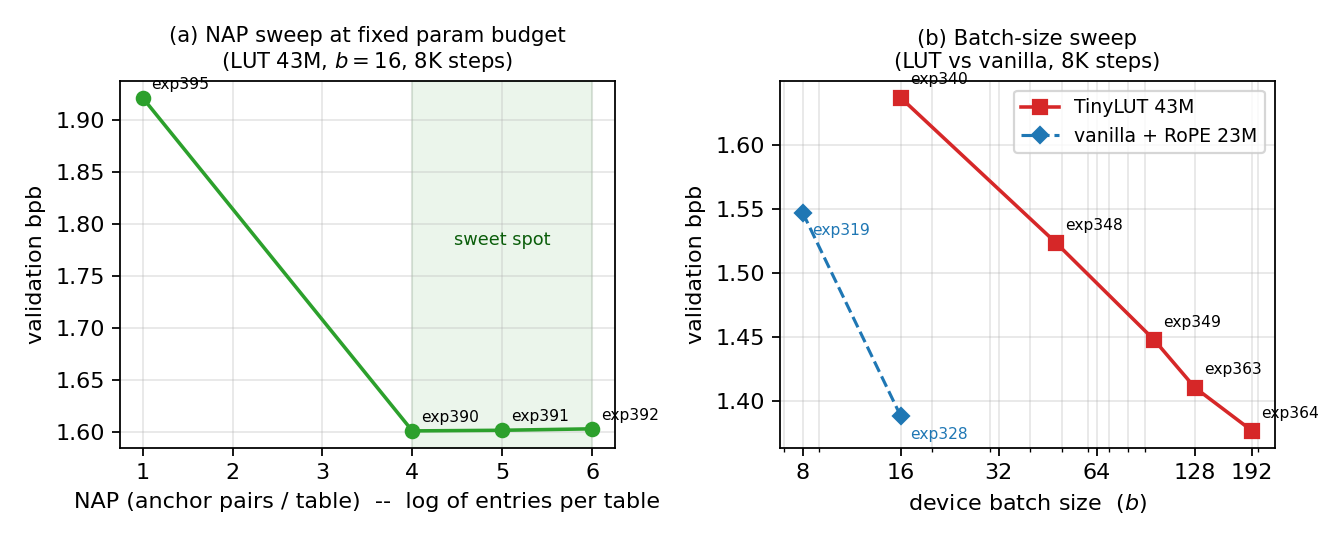
\includegraphics[width=\linewidth]{figs/exp428_nap_batch.png}
\caption{(a) NAP sweep at fixed param budget and $b{=}16$, on a single \texttt{out\_proj} replacement (other LUTs held fixed). NAP $= 1$ is starved of expressivity; NAP $\in \{4, 5, 6\}$ are essentially tied; the shaded band is the working sweet spot. (b) Batch-size sweep at fixed recipe (TinyLUT 43\,M, 8K steps, NAP $= 6$) compared against vanilla + RoPE at the same step budget. The LUT slope is steeper than the vanilla slope; at $b{=}192$ the LUT crosses vanilla.}
\label{fig:nap_batch}
\end{figure}

\paragraph{Practical reading.}
We treat NAP and $b$ as one design pair: pick NAP from the sweet spot to fix the table's expressivity, then scale $b$ as large as memory allows.
None of the orthogonal knobs we tested in the same range (LUT lr sweeps in \texttt{exp353}--\texttt{exp356}, lookahead in \texttt{exp357}, hard-mining in \texttt{exp358}, row-LR EMA in \texttt{exp359}, soft top-$k$ routing in \texttt{exp402}--\texttt{exp403}, input noise in \texttt{exp384}--\texttt{exp385}) moved val bpb by more than $\approx 0.02$ at fixed $(NAP, b)$.
The NAP--batch pair dominates everything else in the slider space.

% ======================================================================
\section{The backward path: soft remains the best we have}
\label{sec:bwd}

The May report's all-soft backward (softmax over the soft-sign comparisons, learnable temperatures, bf16 storage) was the workhorse going into this branch.
We retested it against the cheaper multi-alternatives STE backward with bernoulli flip noise (\texttt{exp386}: $1.6164$ bpb, $\approx 0.012$ worse than the matched soft baseline), the soft top-$k$ score routing variants (\texttt{exp402}, \texttt{exp403}), and a handful of curriculum/STE combinations (\texttt{exp399}, \texttt{exp401}, \texttt{exp415}); all sit within $\pm 0.01$ bpb of the soft baseline at the same recipe.
The fused soft backward remains the best-performing path we have at the bpb numbers in this report; we use it for every LUT in \texttt{exp428}.

One small recipe change went the other way against the prior session: we finally turned the argmax flip-noise off (\texttt{argmax\_noise\_eps}=0).
At $b{=}8$ the small bernoulli flip noise on low-confidence comparisons gave a measurable improvement; at $b \geq 16$ -- on every architecture in this branch -- clean argmax was the same or slightly better (e.g.\ \texttt{exp362} at $b{=}96$, noise $=0$, $1.4296$ bpb vs.\ the matched noise-on \texttt{exp349} at $1.4478$).
Once batch is large enough to give each LUT row a few independent visits per step, the noise stops helping and starts costing.
\texttt{exp428} therefore runs with noise off on every LUT.

% ======================================================================
\section{The architecture, in detail: \texttt{exp428}}
\label{sec:arch}

\paragraph{Block.}
Section~\ref{sec:tiny}'s tiny-LUT seed (\texttt{exp329}\,--\,\texttt{exp342}) used the dual-stream layout from the \texttt{exp303} report -- $E$-carry plus $D$-residual, with V2D/D2V removed -- but with an aggressively small ranking carrier and recipe.
Two changes turn that into the \texttt{exp428} block (Figure~\ref{fig:block}):
\begin{enumerate}[itemsep=1pt, topsep=2pt]
    \item \textbf{Pre-norm with an identity skip on the $E$-stream.} The block reads $\mathtt{ln\_pre}(\mathbf{x}^{\text{lut}}_\ell)$, runs the LUTs and SDPA, and adds the $\mathtt{out\_proj}$ output \emph{back into} $\mathbf{x}^{\text{lut}}_\ell$ before passing it to the next block. This is the standard GPT-2 pre-norm pattern, applied to the ranking carrier. It is the single change that broke us out of the $1.55$ floor on the dual-stream branch (\texttt{exp418}).
    \item \textbf{Fused $\mathtt{qkv\_lut}$ with a shallow $V$-branch.} Q and K come from a single $\mathtt{qkv\_lut}$ that produces $2d_{qk} + d_v$ outputs per head; the last $d_v$ outputs are added into the output of the separate (deeper, wider) $\mathtt{v\_lut}$. The fused table is small (NAP $= 6$, tph $= 64$) and pays a small per-block bandwidth cost in exchange for a cleanly aligned Q/K lookup; the shallow $V$-branch from the same table acts as a residual shortcut for $V$ that lets the deeper $\mathtt{v\_lut}$ specialise.
\end{enumerate}
The post-norm output of the block is fed into $\mathtt{residual\_lut}$ ($\mathbb{R}^E \to \mathbb{R}^D$, NAP $= 6$, tph $= 128$), exactly as in the \texttt{exp303} report; its output is summed into the $D$-residual stream that is LayerNorm'd and passed through a single untied linear $\mathbb{R}^{384} \to \mathbb{R}^{V}$ at the end.

\begin{figure}[!ht]
\centering
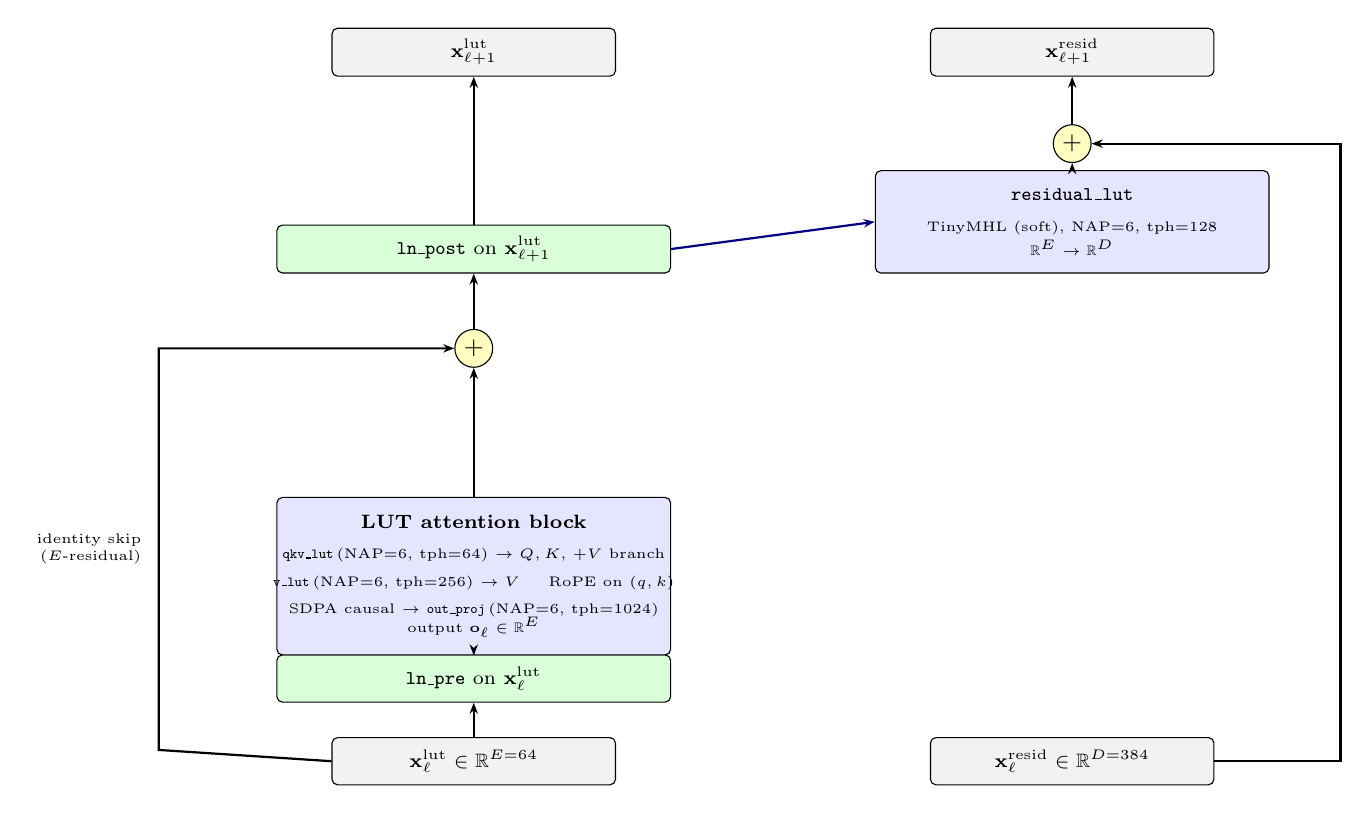
\begin{tikzpicture}[
    x=1cm, y=1cm,
    every node/.style={font=\scriptsize},
    box/.style={rectangle, draw, rounded corners=2pt, align=center, inner sep=4pt, fill=#1, minimum height=0.6cm},
    box/.default=blue!8,
    lut/.style={box=blue!10},
    norm/.style={box=green!15},
    add/.style={circle, draw, inner sep=1.5pt, fill=yellow!25, font=\small, minimum size=0.45cm},
    arr/.style={-{Stealth[length=4pt]}, thick},
    sidearr/.style={-{Stealth[length=4pt]}, thick, blue!50!black},
]
    % --- Column x-coordinates: LEFT for E-stream, RIGHT for D-stream ---
    \def\Lx{-3.8}
    \def\Rx{ 3.8}
    % --- Vertical grid (bottom to top), compact spacing ---
    \def\yA{0.0}   % inputs
    \def\yB{1.05}  % ln_pre
    \def\yC{3.65}  % LUT attention block south (block height ~2.0)
    \def\yD{5.55}  % +adder on E-stream
    \def\yE{6.5}   % ln_post
    \def\yF{8.15}  % +adder on D-stream (after residual_lut joins, rlut top at \yE+1.3=7.8)
    \def\yG{9.0}   % outputs

    % --- Input streams ---
    \node[box=gray!10, minimum width=3.6cm, anchor=south] (xlin)  at (\Lx, \yA)
        {$\mathbf{x}^{\text{lut}}_\ell \in \mathbb{R}^{E=64}$};
    \node[box=gray!10, minimum width=3.6cm, anchor=south] (xrin)  at (\Rx, \yA)
        {$\mathbf{x}^{\text{resid}}_\ell \in \mathbb{R}^{D=384}$};

    % --- Pre-norm ---
    \node[norm, minimum width=5.0cm, anchor=south] (lnpre) at (\Lx, \yB)
        {$\mathtt{ln\_pre}$ on $\mathbf{x}^{\text{lut}}_\ell$};

    % --- LUT attention block (compact, one item per line) ---
    \node[lut, minimum width=5.0cm, minimum height=2.0cm, anchor=south] (blk) at (\Lx, \yC - 2.0) {};
    \node[font=\scriptsize\bfseries, anchor=north] at ([yshift=-3pt]blk.north) {LUT attention block};
    \node[font=\tiny, anchor=north, align=center] at ([yshift=-15pt]blk.north)
        {$\mathtt{qkv\_lut}$\,(NAP=6, tph=64) $\to Q, K$, $+V$ branch};
    \node[font=\tiny, anchor=north, align=center] at ([yshift=-25pt]blk.north)
        {$\mathtt{v\_lut}$\,(NAP=6, tph=256) $\to V$ \;\;\; RoPE on $(q, k)$};
    \node[font=\tiny, anchor=north, align=center] at ([yshift=-35pt]blk.north)
        {SDPA causal $\to$ $\mathtt{out\_proj}$\,(NAP=6, tph=1024)};
    \node[font=\tiny, anchor=south, align=center] at ([yshift=3pt]blk.south)
        {output $\mathbf{o}_\ell \in \mathbb{R}^E$};

    % --- E-stream identity-skip adder ---
    \node[add, anchor=center] (ladd) at (\Lx, \yD) {$+$};

    % --- Post-norm ---
    \node[norm, minimum width=5.0cm, anchor=south] (lnpost) at (\Lx, \yE)
        {$\mathtt{ln\_post}$ on $\mathbf{x}^{\text{lut}}_{\ell+1}$};

    % --- residual_lut on the right column, aligned with lnpost ---
    \node[lut, minimum width=5.0cm, minimum height=1.3cm, anchor=south] (rlut) at (\Rx, \yE) {};
    \node[font=\scriptsize\bfseries, anchor=north] at ([yshift=-3pt]rlut.north)
        {$\mathtt{residual\_lut}$};
    \node[font=\tiny, anchor=north, align=center] at ([yshift=-15pt]rlut.north)
        {TinyMHL (soft), NAP=6, tph=128};
    \node[font=\tiny, anchor=south, align=center] at ([yshift=3pt]rlut.south)
        {$\mathbb{R}^E \to \mathbb{R}^D$};

    % --- D-stream adder ---
    \node[add, anchor=center] (radd) at (\Rx, \yF) {$+$};

    % --- Outputs ---
    \node[box=gray!10, minimum width=3.6cm, anchor=south] (xlout) at (\Lx, \yG)
        {$\mathbf{x}^{\text{lut}}_{\ell+1}$};
    \node[box=gray!10, minimum width=3.6cm, anchor=south] (xrout) at (\Rx, \yG)
        {$\mathbf{x}^{\text{resid}}_{\ell+1}$};

    % --- Wiring (E-stream main path) ---
    \draw[arr] (xlin.north)  -- (lnpre.south);
    \draw[arr] (lnpre.north) -- (blk.south);
    \draw[arr] (blk.north)   -- (ladd.south);
    \draw[arr] (ladd.north)  -- (lnpost.south);
    \draw[arr] (lnpost.north) -- (xlout.south);

    % --- Identity skip: bypass the WHOLE block on its left, well clear of node text ---
    \coordinate (skipL) at (\Lx - 4.0, \yA + 0.45);
    \coordinate (skipU) at (\Lx - 4.0, \yD);
    \draw[arr, thick] (xlin.west) -- (skipL) -- (skipU) -- (ladd.west);
    \node[font=\tiny, anchor=east, align=right] at ($(skipL)!0.5!(skipU) + (-0.1, 0)$)
        {identity skip\\($E$-residual)};

    % --- Cross-stream: ln_post output taps residual_lut input ---
    \draw[sidearr] (lnpost.east) -- (rlut.west);

    % --- D-stream ---
    % x_resid bypasses residual_lut on the RIGHT, then joins the + adder from the right
    \draw[arr, thick] (xrin.east) -| ++(1.6, 0) |- (radd.east);
    \draw[arr] (rlut.north)  -- (radd.south);
    \draw[arr] (radd.north)  -- (xrout.south);
\end{tikzpicture}
\caption{One block of the \texttt{exp428} dual-stream LUT transformer. \emph{Left column}: the $E$-stream ranking carrier flows through pre-norm $\to$ LUT attention block $\to$ identity-skip adder $\to$ post-norm. \emph{Right column}: the $D$-stream real-valued residual receives a contribution from $\mathtt{residual\_lut}$, which reads the post-normed $E$-stream and projects $\mathbb{R}^E \to \mathbb{R}^D$. The two changes vs.\ \texttt{exp303}: the GPT-2-style pre-norm + identity skip on the $E$-stream (replacing the May report's V2D/D2V tail), and a fused $\mathtt{qkv\_lut}$ whose last $d_v$ outputs are added into the separate $\mathtt{v\_lut}$ output to form a shallow $V$-branch. After the last block, $\mathbf{x}^{\text{resid}}$ is LayerNorm'd and projected by an untied linear $\mathbb{R}^{384} \to \mathbb{R}^{V}$. No FFN; no weight decay on LUT weights, token or position embeddings.}
\label{fig:block}
\end{figure}

\paragraph{Lineage.}
Each step between the pre-residual tiny-LUT baseline and \texttt{exp428} was tested in isolation as a single-knob change against the immediately preceding sibling:

\begin{center}\small
\begin{tabular}{lllr}
\toprule
Run & Single-knob change vs.\ predecessor & Params & val bpb \\
\midrule
\texttt{exp407} & pre-residual baseline (TinyLUT $E{=}48$)           & $43.1$\,M & $1.6038$ \\
\texttt{exp419} & + $E$-residual identity skip + qkv\_only           & $64.9$\,M & $1.5426$ \\
\texttt{exp423} & + separate $\mathtt{v\_lut}$                      & $43.1$\,M & $1.5459$ \\
\texttt{exp424} & + $E{=}64$                                          & $46.7$\,M & $1.5390$ \\
\texttt{exp425} & + $\mathtt{v\_tph}\,256$                            & $51.4$\,M & $1.5298$ \\
\texttt{exp427} & + tph $\times 2$ on $\mathtt{out\_proj}$, $\mathtt{residual\_lut}$ & $78.8$\,M & $1.5046$ \\
\textbf{\texttt{exp428}} & + $\mathtt{qkv\_tph} \times 2$            & $\mathbf{89.4}$\,\textbf{M} & $\mathbf{1.4983}$ \\
\bottomrule
\end{tabular}
\end{center}
The $E$-residual identity skip is the discontinuous step ($-0.061$ bpb); the remainder is a sequence of capacity widenings, each $0.005$--$0.025$ bpb at low parameter cost.

\paragraph{Headline result.}
At 8K steps, $b{=}16$, on the matched recipe:
\begin{center}\small
\begin{tabular}{llrr}
\toprule
Run & What & Params & val bpb \\
\midrule
\texttt{exp328} & vanilla + RoPE                              & $23.4$\,M & $1.388$ \\
\texttt{exp407} & dual-stream LUT (pre-residual, baseline)     & $43.1$\,M & $1.604$ \\
\textbf{\texttt{exp428}} & dual-stream LUT (this report) & $\mathbf{89.4}$\,\textbf{M} & $\mathbf{1.498}$ \\
\midrule
\multicolumn{4}{l}{\emph{at larger batch / longer horizon (same architecture):}} \\
\texttt{exp429}  & exp428 arch, $b{=}32$, 8K            & $89.4$\,M & $1.418$ \\
\textbf{\texttt{exp430}}  & \textbf{exp428 arch, $b{=}48$, 24K}              & $89.4$\,M & $\mathbf{1.285}$ \\
\bottomrule
\end{tabular}
\end{center}

The lineage closes a $0.106$ bpb gap from the pre-residual baseline ($1.604 \to 1.498$) at less than $2\times$ the parameter count.
Against vanilla on the matched 8K / $b{=}16$ budget, \texttt{exp428} is $0.110$ bpb behind ($1.498$ vs.\ $1.388$).
At $b{=}32$ the same architecture closes that to $0.030$ bpb behind vanilla \texttt{exp328}; and at $b{=}48$, 24K, \texttt{exp430} finishes at $\mathbf{1.285}$ bpb -- $0.032$ bpb behind the long-horizon vanilla \texttt{exp416} ($1.253$), on a model that fits in $\sim 90$\,M parameters.
This is the closest a LUT model has come to vanilla at matched compute in this project.
Figure~\ref{fig:val} shows the per-step trajectories.

\begin{figure}[!ht]
\centering
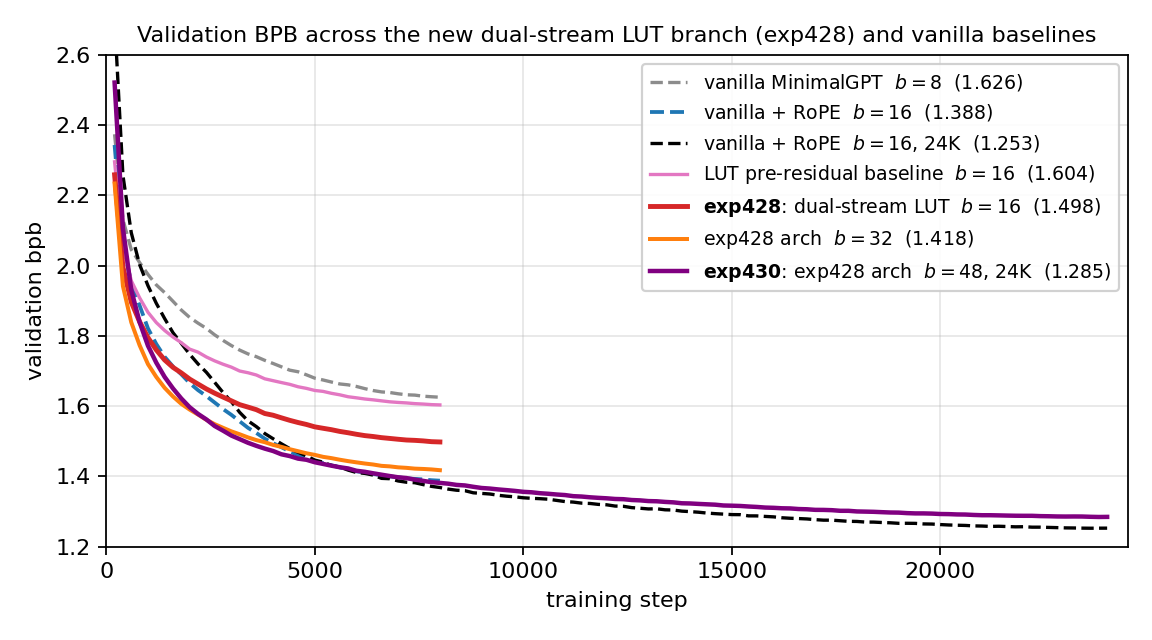
\includegraphics[width=0.88\linewidth]{figs/exp428_val_bpb.png}
\caption{Validation bpb against training step for the LUT branch (solid) and vanilla + RoPE baselines (dashed). The pre-residual LUT baseline \texttt{exp407} sits at $1.604$; \texttt{exp428} brings it to $1.498$ at the same $b{=}16$, 8K budget; \texttt{exp429} (same architecture, $b{=}32$) reaches $1.418$; \texttt{exp430} (same architecture, $b{=}48$, 24K) finishes at $1.285$, within $0.032$ bpb of vanilla \texttt{exp416} on the matched 24K horizon.}
\label{fig:val}
\end{figure}

% ======================================================================
\section{What did not work}
\label{sec:failures}

\paragraph{Distillation from vanilla.}
The natural way to attack the residual vanilla advantage was to distil from \texttt{exp416} (vanilla + RoPE 24K, $1.253$ bpb) into the \texttt{exp428}-shaped LUT model.
We tried four variants -- a head-only distillation against the teacher's softmax (\texttt{exp431}), a layer-aligned representation distillation (\texttt{exp432}), and two longer-horizon student-only runs at $b{=}64$ (\texttt{exp433}, constant LR; \texttt{exp434}, cosine).
None caught up to even the cross-entropy-trained \texttt{exp428}.
The current diagnosis is that the teacher's logits are too low-temperature for the LUT student's discrete routing to follow informatively, and that the LUT block's per-token gradient sparsity (Section~\ref{sec:nap_batch}) compounds the distillation noise.
We have parked this line until either the LUT model's per-token routing is more entropic at convergence or the teacher's logits are temperature-softened in a principled way.

\paragraph{Larger / smaller table sweeps that did not help.}
\texttt{exp390}--\texttt{exp392} confirmed the NAP sweet spot (Section~\ref{sec:nap_batch}); going below or above it produced no surprises.
The earlier mixture-of-NAPs out\_proj experiments (\texttt{exp387}--\texttt{exp389}) and the curriculum-NAP schedules (\texttt{exp396}--\texttt{exp400}, \texttt{exp415}) failed to beat the single-NAP baseline at fixed budget.
Pruning $\mathtt{v\_lut}$ entirely (\texttt{exp404}--\texttt{exp406}) costs only $\sim 0.01$ bpb at $b{=}16$ and scales cleanly with $b$, so the shallow-$V$ branch in $\mathtt{qkv\_lut}$ is doing most of the per-token $V$ work; \texttt{exp428} keeps a separate $\mathtt{v\_lut}$ because the cost-to-bpb trade is still favourable, but it is the next obvious thing to remove if bandwidth becomes binding.

% ======================================================================
\section{Bandwidth}
\label{sec:bandwidth}

The May report's bandwidth methodology (Sec.\ ``Bandwidth'', Table 1 there) carries over unchanged.
For \texttt{exp428}, the per-token weight reads decompose as in Table~\ref{tab:bw}.
We strip the unembedder from both totals -- the LUT model and the vanilla baseline share the same dense untied linear $\mathbb{R}^{384} \to \mathbb{R}^{V}$, and it dominates both budgets in absolute terms.

\begin{table}[!ht]
\caption{Per-token weight reads (fp32 forward, no batch amortisation). Trunk reads include all per-layer projections summed over six layers; for the LUT model these are LUT lookups, for vanilla they are dense matmul reads.}
\label{tab:bw}
\centering\small
\begin{tabular}{lrr}
\toprule
Component & Vanilla + RoPE (\texttt{exp328}) & exp428 LUT \\
\midrule
$\mathtt{qkv\_lut}$ trunk read / layer  & --- & $55{,}296$ \\
$\mathtt{v\_lut}$ trunk read / layer    & --- & $24{,}576$ \\
$\mathtt{out\_proj}$ trunk read / layer  & --- & $65{,}536$ \\
$\mathtt{residual\_lut}$ trunk read / layer & --- & $49{,}152$ \\
Dense per-layer reads & $1{,}769{,}472$ & --- \\
\midrule
Trunk total, six layers & $10{,}616{,}832$ \,($\sim$$42$\,MB)  & $1{,}167{,}360$ \,($\sim$$4.7$\,MB) \\
Embedding lookups       & $\sim$$10^3$                         & $\sim$$10^3$ \\
\textbf{Trunk + emb (no unembedder)} & $\sim 10.6\,\mathbf{M}$ & $\sim 1.2\,\mathbf{M}$ \\
Unembedder (Linear $384 \to V$) & $12{,}582{,}912$ ($\sim$$50$\,MB) & $12{,}582{,}912$ ($\sim$$50$\,MB) \\
\bottomrule
\end{tabular}
\end{table}

After subtracting the shared unembedder term, the LUT trunk reads $\sim 9\times$ fewer weights per token than the vanilla trunk -- and across the family of compact-recipe LUT models we trained in this branch the ratio sits in the $10$--$20\times$ range, depending on which projections are present.
That is the architecture's selling point in this regime: at $\sim 4\times$ the trunk parameter count, the LUT trunk reads roughly an order of magnitude less weight memory per token than the vanilla trunk does, because each per-table read scales with $\mathrm{tph}$ rather than with $E^2$.
The remaining bandwidth gap to vanilla is concentrated in the dense unembedder; folding that into a LUT-family module is the natural next architectural target.

% ======================================================================
\section*{Conclusion}

\begin{enumerate}[itemsep=2pt, topsep=4pt]
\item \textbf{RoPE embeddings.} A simple idea that works well, and -- surprisingly -- works with LUT transformers as well. Following Occam's razor we decided to switch the baseline: vanilla + RoPE $b{=}16$ $= 1.3882$ (the new 8K bar).
\item \textbf{Tiny model thesis.} All our previous models were very big. We decided to build a tiny model that would be competitive. We discovered that after a certain point large investments in table count lead to very modest profit, so we decided not to go above $100$\,M parameters. We tried a lot of different configurations. It is important to notice that all LUT models we tried are $10$ to $20$ times better than vanilla in terms of bandwidth after subtracting the unembedder bandwidth from both estimates.
\item \textbf{Batch and NAP.} We conducted a lot of experiments with batches of different size. LUT models benefit from bigger batches even more than vanilla because bigger batches are the only way to attack the sparsity of the LUT gradients. It looks like we are dealing with some kind of trade-off: decreasing the size of tables (NAP) you lower the expressivity of the model but at the same time you decrease sparsity and gradients become better. On the opposite, if you make tables bigger you increase the potential expressivity but gradients become very sparse and you need very big batches to train. Sweet spot is in the middle. Around NAP $= 4$--$6$.
\item \textbf{Backward path.} We did additional tests trying to improve LUT gradients backward path, but still our softmax-over-soft-signs backward model remains the best.
\item \textbf{Residual path in the LUT stream.} At some point we discovered that adding the residual path into the LUT stream helps a lot, and finally we came up with the architecture presented in \texttt{exp428}--\texttt{exp430} that allowed us to pass below $1.5$ bpb at $b{=}16$, 8K steps, and reach $1.285$ at $b{=}48$, 24K -- within $0.032$ bpb of vanilla on the matched 24K horizon.
\item \textbf{Distillation.} We tried to distill information from a well-trained vanilla transformer into LUT models, but all our attempts failed.
\item \textbf{Overall.} All our findings led to better loss values and we are much closer to vanilla than before, but still vanilla converges faster and reaches better loss values at the same number of processed tokens.
\end{enumerate}

\end{document}
